\chapter{Modification de la régulation}

\section{Introduction}
Ce chapitre traite les modifications apportées à la régulation de courant ainsi que la nouvelle régulation de position réalisées au cours de ce travail de bachelor. Le schéma bloc décrivant le nouveau système est présenté dans l'\autoref{fig:SchemaBlocTot}:

\begin{figure}[H]
    \centering
    \includesvg[width=1\linewidth]{assets/content/12-ModifRegulation/SchemaRegTot}
    \caption{Principe de la régulation de position-courant employé}
    \label{fig:SchemaBlocTot}
\end{figure}

La régulation de position en Single Input Single Output (SISO) n'ayant pas fait ses preuves, une régulation en Multiple Input Multiple Output (MIMO) a été envisagée et réalisée. Les détails de cette méthode sont décrits dans les sections à venir. Ce chapitre permet également de statuer sur l'hypothèse de la \autoref{sec:Hypothese} concernant une erreur introduite lors de la phase de synthèse des régulateurs (\autoref{subsec:RegPIError}).

\section{Analyse de la régulation de courant}

\subsection{Changement des valeurs d'inductances}
Suite a la découverte des nouvelles valeurs d'inductances, il est néscessaire de les inclures dans le système a régler. Ceux-ci apparaissent principalement dans l'équation du système $G_{ui}$. Pour rappel, le système $G_{ui}$ est décrit comme telle :

\begin{equation}
    G_{ui}(s) = K_{ui}\cdot\frac{s}{1 + a_1 \cdot s + a_2\cdot s^2}
\end{equation}

Avec :

\begin{equation*}
    \left\{ \begin{aligned}
         & K_{ui} = \frac{m}{L_n^2}\cdot \left(\frac{\delta_n}{i_n} \right)^2                     \\
         & a_1 = \frac{m\cdot R}{L_n^2}\cdot \left(\frac{\delta_n}{i_n} \right)^2                 \\
         & a_2 = \frac{m}{L_n}\cdot\left(\frac{\delta_n}{i_n^2}\right)^2 = \frac{L_n}{R}\cdot a_1
    \end{aligned} \right.
\end{equation*}

En reprenant les résultats obtenus dans le \autoref{tab:mesures_2mm}, il est possible de les intégrer dans le script Matlab réalisé par Yersin \cite{Yersin} comme suit :

\begin{minted}{matlab}
    R1      = 1.172409;                    % résistance de la bobine 1
    R2      = 1.365961;                    % résistance de la bobine 2
    R3      = 1.228376;                    % résistance de la bobine 3
    R4      = 1.336800;                    % résistance de la bobine 4
    L_n1    = 7.741565e-3;                 % inductance nominale 1
    L_n2    = 8.647352e-3;                 % inductance nominale 2
    L_n3    = 7.699234e-3;                 % inductance nominale 3
    L_n4    = 7.749885e-3;                 % inductance nominale 4
\end{minted}

\subsection{Erreur}
\label{subsec:RegPIError}
Lors d'une analyse de la régulation de courant, une erreur majeure a été découverte : le système à régler n'est pas correctement synthétisé. En effet, la multiplication par la constante $K_{ui}$ a été omise, comme le démontre ce code :

\begin{minted}{matlab}
%% Inducteur Linéarisé autour de d_n = 2mm (avec terme en delta_d négliger p.12 journal)

Kui     = (d_n/i_n)^2*(m/L_n^2);
a1      = (d_n/i_n)^2*(m*R/L_n^2);
a2      = (d_n/i_n)^2*(m/L_n);

num     = [1 0];
den     = [a2 a1 1];
Gui     = tf(num,den); % Manque Kui
\end{minted}

Cette omission modifie significativement le comportement du système à régler. L'hypothèse de la \autoref{sec:Hypothese} selon laquelle une erreur a été introduite lors de la phase de synthèse des régulateurs est ainsi confirmée. Les courbes montrent que le gain initial réel débute à environ $-40$~dB et non à 0~dB :

\begin{figure}[H]
    \centering
    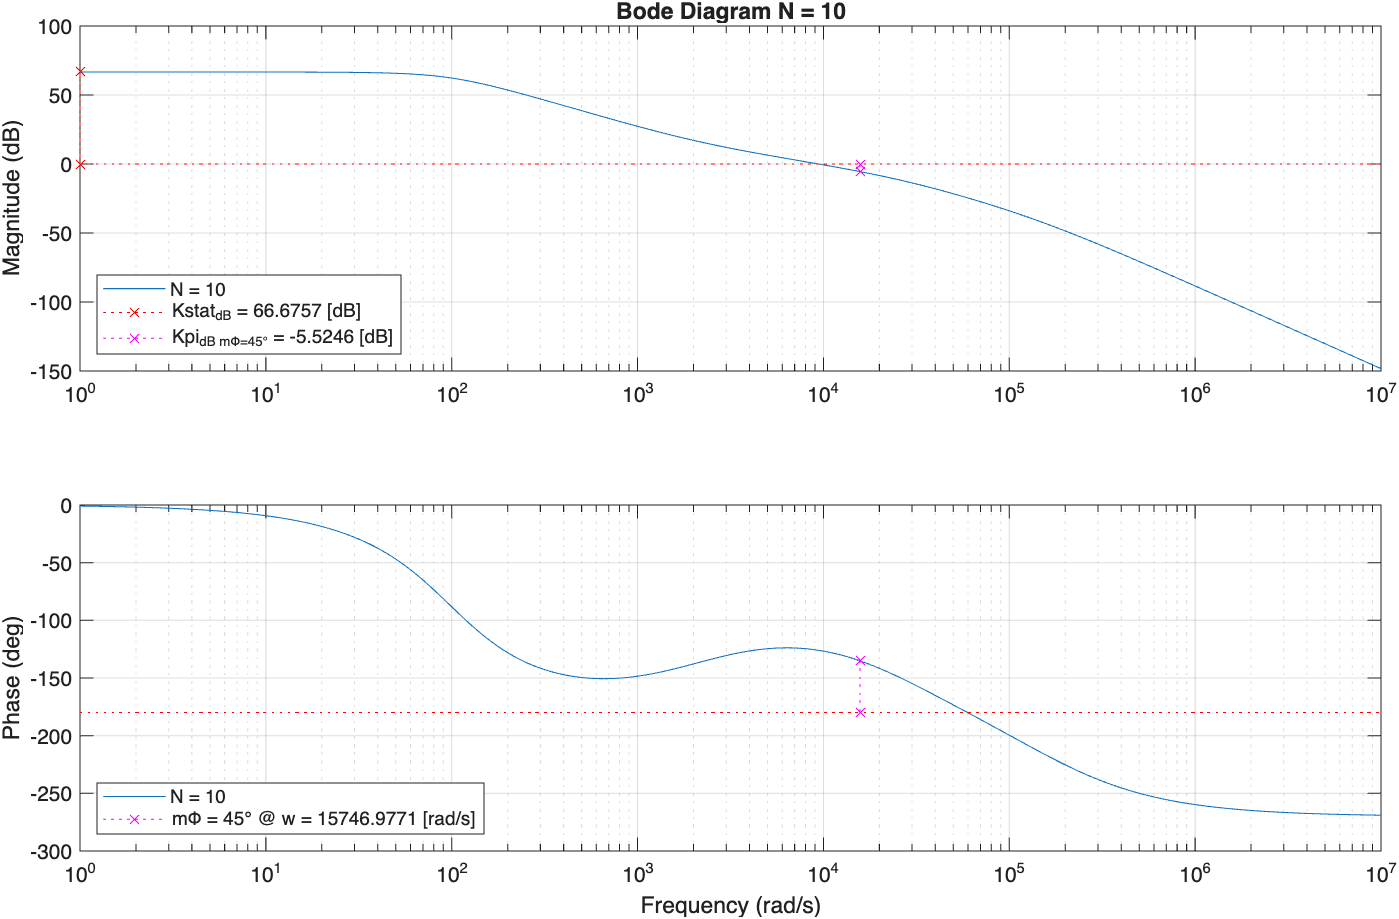
\includegraphics[width=1\linewidth]{assets/content/12-ModifRegulation/RegCour/BodeKpiFaux.png}
    \caption{Système à régler sans la constante multiplicative $K_{ui}$}
\end{figure}

\begin{figure}[H]
    \centering
    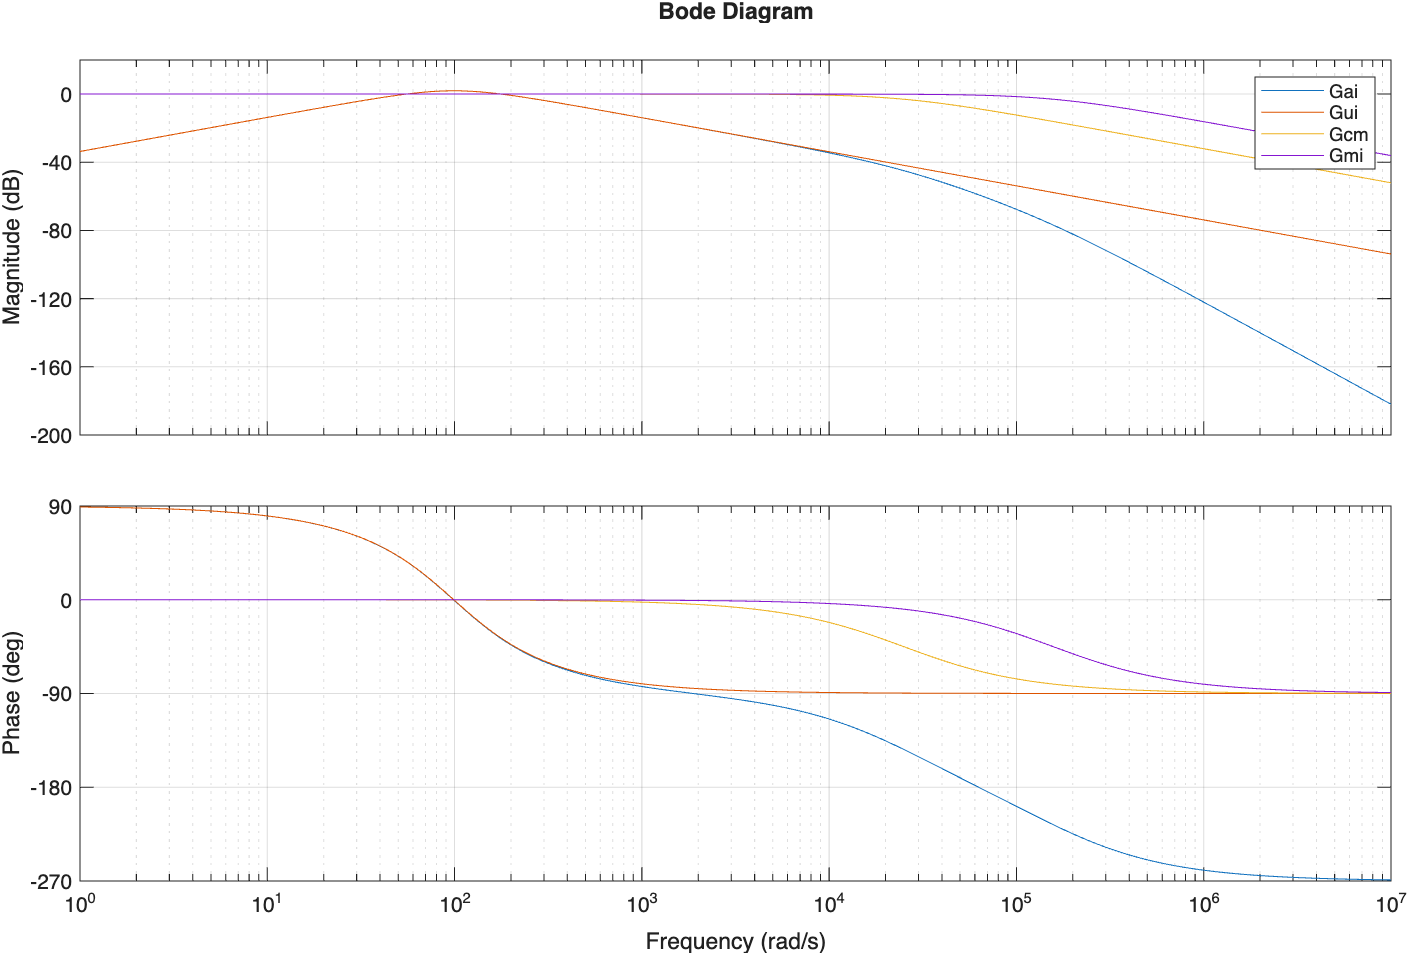
\includegraphics[width=1\linewidth]{assets/content/12-ModifRegulation/RegCour/BodeGaiVrai.png}
    \caption{Système à régler avec la constante multiplicative $K_{ui}$}
\end{figure}

Lors de la même synthèse que précédemment (voir l'\autoref{sec:RegCourPrec}), il est possible de réaliser une comparaison des paramètres avec et sans la prise en compte de la constante $K_{ui}$ :

\begin{table}[H]
    \centering
    \begin{tabular}{lcc}
        \hline
        \textbf{Paramètre} & \textbf{Sans $K_{ui}$} & \textbf{Avec $K_{ui}$} \\ \hline
        $\tau_{ii}$        & $4.63 \cdot 10^{-4}$   & $4.63 \cdot 10^{-4}$   \\
        $K_{pi}$           & $1.89$                 & $90.96$                \\
        $\tau_{iBF}$       & $7.83 \cdot 10^{-5}$   & $7.83 \cdot 10^{-5}$   \\ \hline
    \end{tabular}
    \caption{Comparaison des paramètres avec et sans intégration de $K_{ui}$}
    \label{tab:comparatif_kui}
\end{table}

L'analyse de ces données montre que seule la valeur du gain $K_{pi}$ est modifiée. L'introduction d'une constante n'exerce aucune influence sur la phase du système, son déphasage propre étant nul. Ce comportement est confirmé par la \autoref{fig:BodeKpiFaux} et la \autoref{fig:BodeKpiVrai} :

\begin{figure}[H]
    \centering
    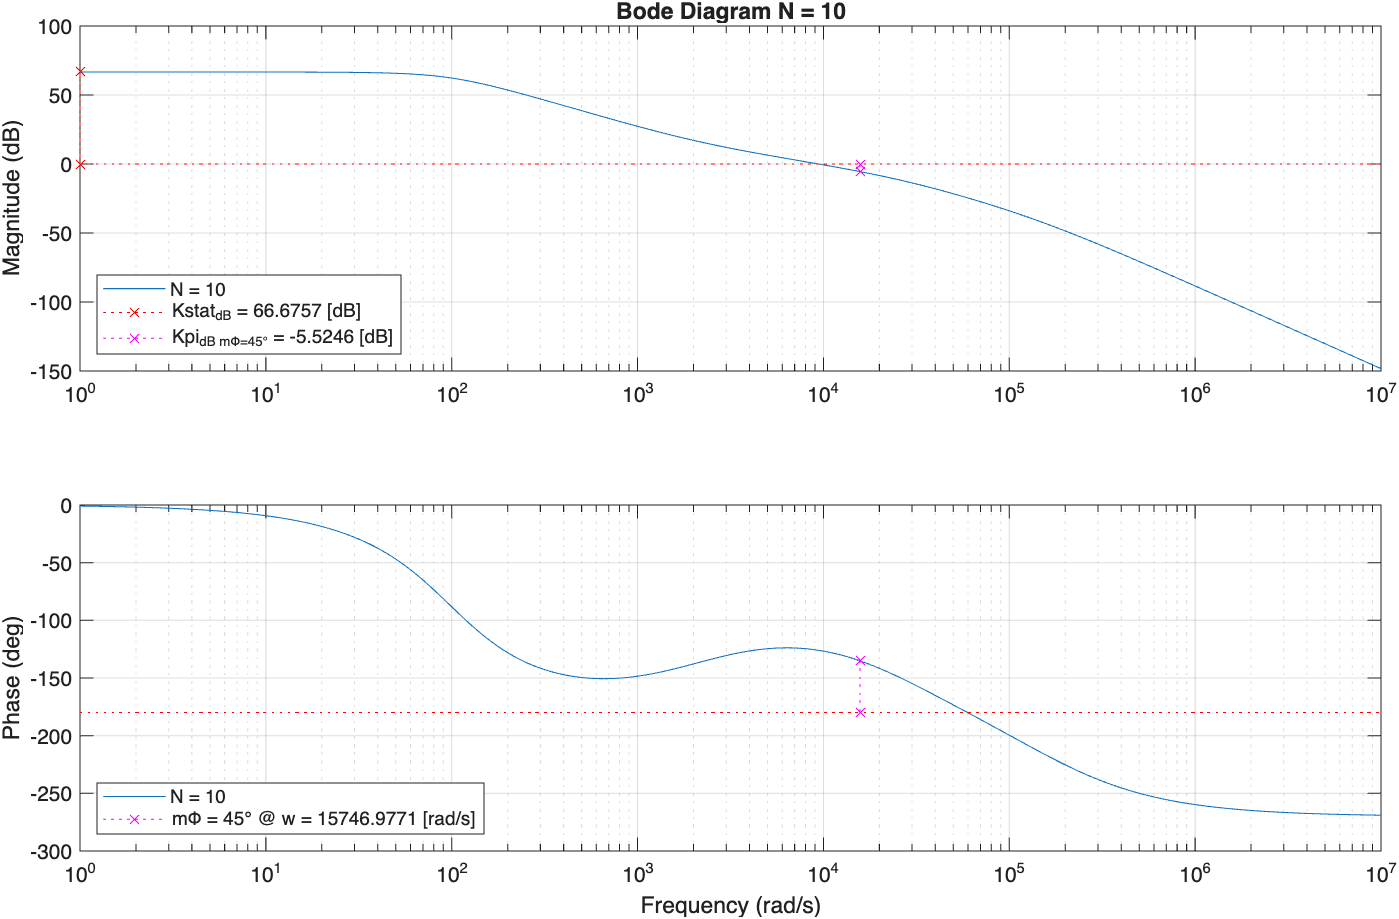
\includegraphics[width=1\linewidth]{assets/content/12-ModifRegulation/RegCour/BodeKpiFaux.png}
    \caption{Identification du gain $K_{pi}$ sans la constante multiplicative}
    \label{fig:BodeKpiFaux}
\end{figure}

\begin{figure}[H]
    \centering
    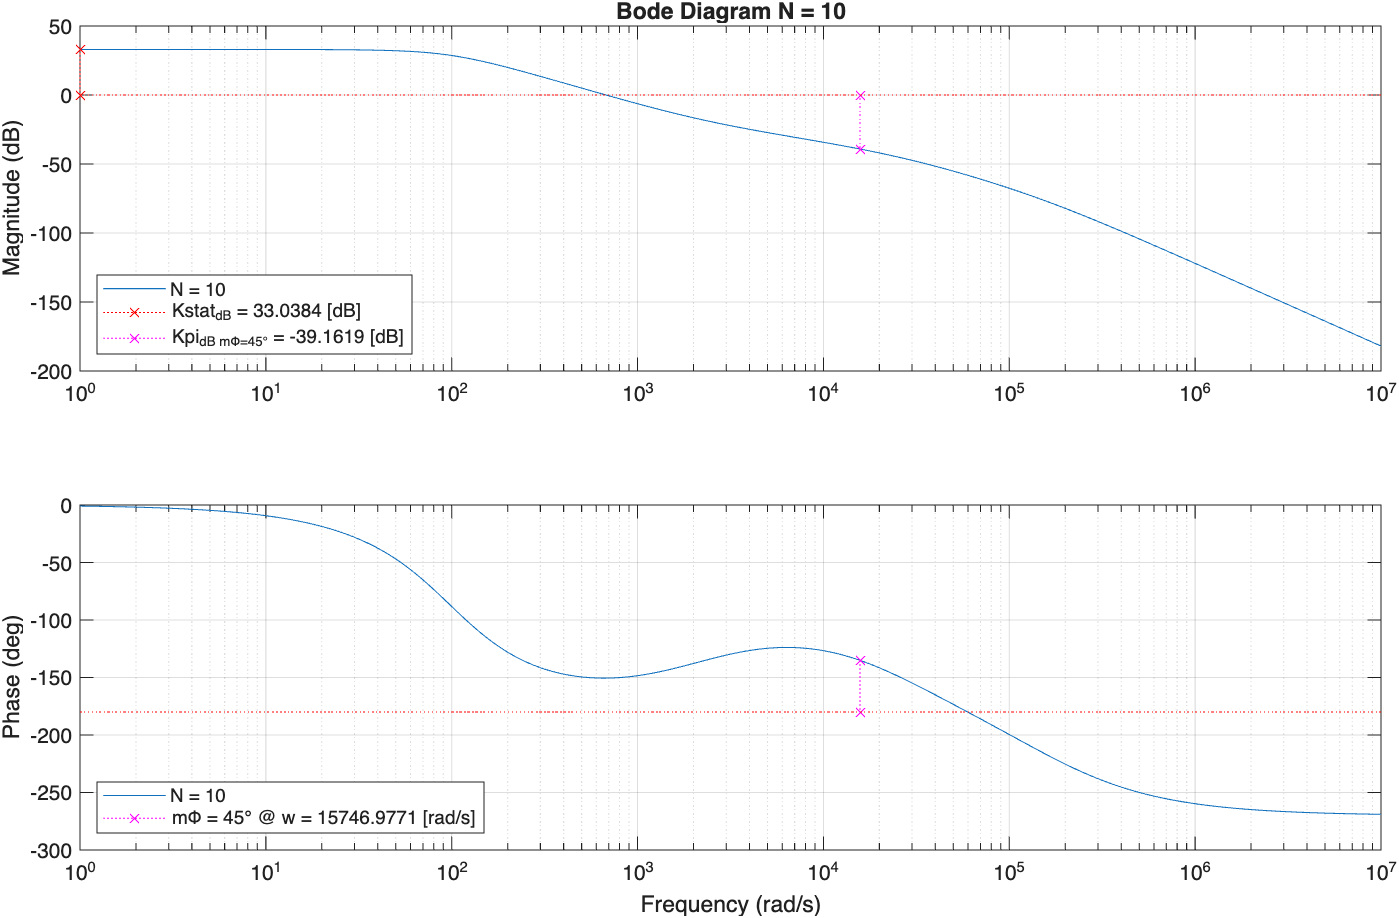
\includegraphics[width=1\linewidth]{assets/content/12-ModifRegulation/RegCour/BodeKpiVrai.png}
    \caption{Identification du gain $K_{pi}$ avec la constante multiplicative}
    \label{fig:BodeKpiVrai}
\end{figure}

Lors de l'implémentation expérimentale, l'introduction de la valeur théorique de 90.96 engendre un plaquage franc de la maquette contre le rail de guidage. Ce phénomène s'explique par le fait que l'étage de puissance a été initialement dimensionné pour le gain inférieur (de l'ordre de 1.89). Avec un gain de 90, une faible erreur statique génère immédiatement une commande en tension saturée. Bien que les limites matérielles du système saturent physiquement la commande à 48~V et 3.5~A, la dynamique excessive requise par ce gain élevé déstabilise le comportement. Les essais physiques mettent en évidence un fonctionnement plus stable pour un gain $K_{pi}$ proche de 1.88. Il est nécessaire de chercher une valeur de $K_{pi}$ fixe convenant au système. Cela aura dès lors un impact sur l'approximation de la boucle fermée qui, n'atteignant jamais la marge de phase désirée, sera beaucoup plus lente que prévu.

Il a alors été décidé de fixer la valeur de $K_{pi}$ à 2 pour chaque inducteur. Cette valeur a été déterminée en essayant de multiples valeurs avec le système en marche. Une fois cette valeur définie, il est nécessaire d'analyser le système en boucle fermée en réalisant un saut indiciel, démontré dans la \autoref{fig:SautInd2} :

\begin{figure}[H]
    \centering
    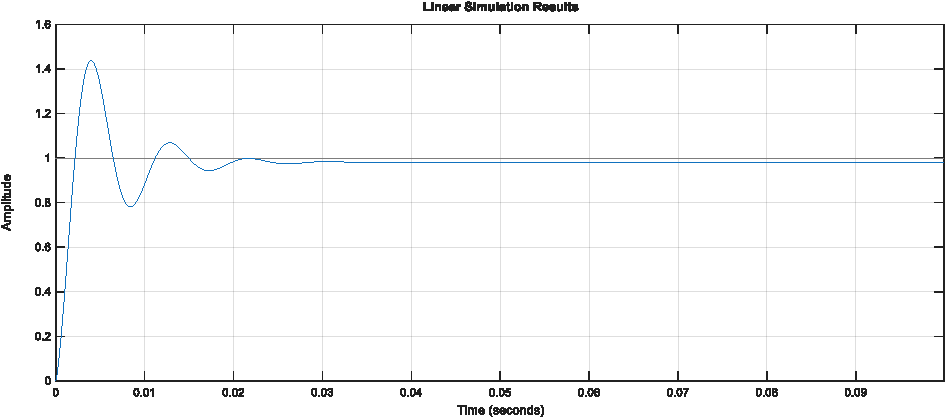
\includegraphics[width=1\linewidth]{assets/content/12-ModifRegulation/RegCour/SautInd1.pdf}
    \caption{Saut indiciel avec $K_{pi}$ fixé à 2 pour l'inducteur 1}
    \label{fig:SautInd2}
\end{figure}

L'erreur donnée pour l'inducteur 1 est de 1.84\%.

Afin de diminuer l'erreur et en se basant sur la \autoref{fig:Erreur}, un $N$ valant 7 a été retenu. Avec cette nouvelle valeur, le saut indiciel devient :

\begin{figure}[H]
    \centering
    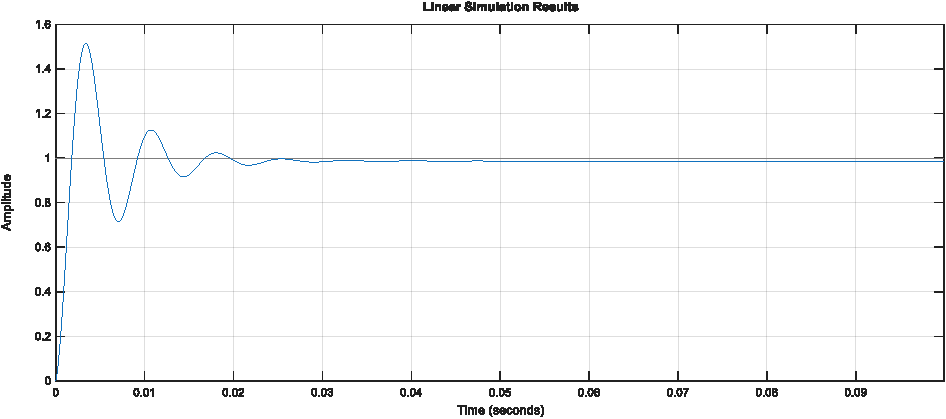
\includegraphics[width=1\linewidth]{assets/content/12-ModifRegulation/RegCour/SautInd2.pdf}
    \caption{Saut indiciel avec $N$ fixé à 7}
    \label{fig:SautInd3}
\end{figure}

L'erreur donnée pour l'inducteur 1 est de 1.29\%.

L'erreur a bel et bien diminué. Il est dès lors possible de rechercher la nouvelle valeur de $\tau_{iBF}$. Pour cela, le script tourna plusieurs fois afin de déterminer la valeur de cette constante de temps. Ceci donna alors les valeurs suivantes par inductance :

\begin{equation*}
    \tau_{iBF1} = 1.60 \text{ms}\quad \tau_{iBF2} = 1.68 \text{ms} \quad \tau_{iBF3} = 1.60 \text{ms} \quad \tau_{iBF4} = 1.60 \text{ms}
\end{equation*}

Comme constater la valeur de $\tau_{iBF}$ est bien plus grande que celle définit pour une marge de phase a 45°. Dès lors une valeur moyenne sera employer pour la synthèse de la régulation de position puisque les 4 valeurs sont proches l'une de l'autre donnant alors :

\begin{equation}
    \tau_{iBF,moy} = 1.62 \text{ms}
\end{equation}

\section{Régulation de positions}
La régulation SISO précédente traite chaque inducteur comme un système indépendant. Chaque boucle mesure son propre entrefer et calcule sa propre force sans tenir compte des trois autres. Or les quatre inducteurs portent la même plaque rigide. Lorsque l'inducteur 1 augmente sa force, il ne lève pas uniquement son coin mais fait pivoter toute la plaque, ce qui modifie aussi les entrefers des inducteurs 2, 3 et 4. Les quatre boucles se perturbent donc en permanence.

L'idée de la régulation MIMO est de ne plus réguler quatre entrefers indépendants mais directement les mouvements de la plaque. Une plaque rigide qui ne se déplace que verticalement possède trois mouvements possibles, appelés modes :

\begin{itemize}
    \item Le pompage : la plaque monte ou descend en restant horizontale.
    \item Le tangage : la plaque pivote autour de son axe $Y$, l'avant descend pendant que l'arrière monte (ou inversement).
    \item Le roulis : la plaque pivote autour de son axe $X$, la gauche descend pendant que la droite monte (ou inversement).
\end{itemize}

Les déplacements horizontaux et la rotation autour de l'axe vertical ne sont pas régulés. De légers mouvements restent possibles dans ces directions, mais aucun capteur ne permet d'y connaître la position. Ces degrés de liberté sont de toute façon bloqués par le guidage mécanique.

La régulation de position suit dès lors le principe de la \autoref{fig:NewSchemaBlocPos} :

\begin{figure}[H]
    \centering
    \includesvg[width=1\linewidth]{assets/content/12-ModifRegulation/RegPos/SchemaBloc}
    \caption{Principe de la régulation MIMO}
    \label{fig:NewSchemaBlocPos}
\end{figure}

\subsection{Remarque}
Par manque de temps, l'intelligence artificielle a été employée pour générer le script calculant les coefficients de la régulation de position.

\subsection{Définition de la géométrie}
La nouvelle régulation nécessite de définir le centre de gravité de la partie lévitante. Il est supposé au centre de la plaque :

\begin{figure}[H]
    \centering
    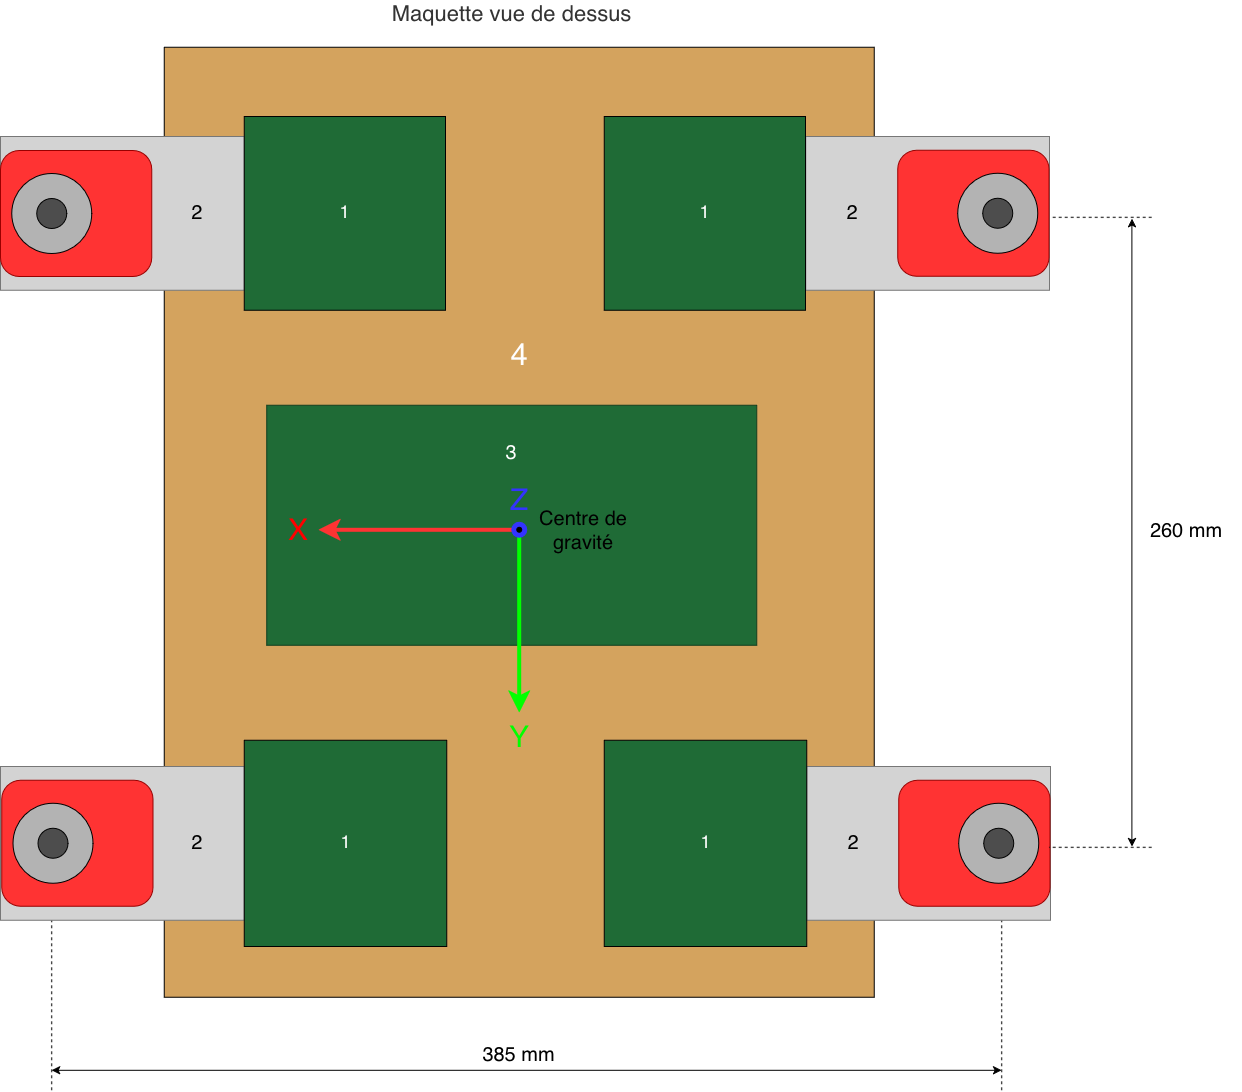
\includegraphics[width=1\linewidth]{assets/content/12-ModifRegulation/RegPos/VueDessus.png}
    \caption{Vue de dessus avec le système d'axe}
    \label{fig:VueDessus}
\end{figure}

Le repère 1 désigne les cartes de puissance, 2 les profilés en aluminium, 3 la carte principale et 4 la plaque en bois.

Les cotes de la \autoref{fig:VueDessus} donnent l'écart entre les pieds. La distance entre deux inducteurs est de 280~mm sur l'axe X et de 260~mm sur l'axe Y.

La position des inducteurs par rapport au centre de gravité est donnée par le \autoref{tab:geom-inducteurs}, où $i$ désigne le numéro de l'inducteur :

\begin{table}[H]
    \centering
    \begin{tabular}{clcc}
        \toprule
        \textbf{Inducteur} & \textbf{Position} & \textbf{$x_i$ [m]} & \textbf{$y_i$ [m]} \\
        \midrule
        1                  & avant-gauche      & $+0.140$           & $+0.130$           \\
        2                  & avant-droit       & $+0.140$           & $-0.130$           \\
        3                  & arrière-gauche    & $-0.140$           & $+0.130$           \\
        4                  & arrière-droit     & $-0.140$           & $-0.130$           \\
        \bottomrule
    \end{tabular}
    \caption{Positions des inducteurs par rapport au centre de gravité}
    \label{tab:geom-inducteurs}
\end{table}

La position de la plaque est décrite par trois grandeurs :

\begin{itemize}
    \item $\bar\delta$ : l'entrefer moyen (pompage) [m]
    \item $\theta$ : l'angle de tangage [rad]
    \item $\varphi$ : l'angle de roulis [rad]
\end{itemize}

Comme précédemment, l'entrefer diminue lorsque la partie lévitante monte.

Considérons l'inducteur $i$ situé aux distances $x_i$ et $y_i$. Lorsque la plaque tourne d'un angle de tangage $\theta$, le coin en $x_i$ se déplace verticalement de $x_i\cdot\sin(\theta)$. Les angles restant très petits, l'approximation $\sin(\theta)\approx\theta$ est admise. Le déplacement vaut alors simplement $x_i\cdot\theta$.

Le même principe s'applique au roulis avec la distance $y_i$.

L'entrefer de l'inducteur $i$ est donc la somme de trois termes :

\begin{equation}
    \delta_i = \bar\delta + x_i\cdot\theta + y_i\cdot\varphi
\end{equation}

Appliquée aux quatre inducteurs, cette relation donne :

\begin{equation*}
    \left\{ \begin{aligned}
         & \delta_1 = \bar\delta + x_1\cdot\theta + y_1\cdot\varphi = \bar\delta + 0.14\cdot\theta + 0.13\cdot\varphi \\
         & \delta_2 = \bar\delta + x_2\cdot\theta + y_2\cdot\varphi = \bar\delta + 0.14\cdot\theta - 0.13\cdot\varphi \\
         & \delta_3 = \bar\delta + x_3\cdot\theta + y_3\cdot\varphi = \bar\delta - 0.14\cdot\theta + 0.13\cdot\varphi \\
         & \delta_4 = \bar\delta + x_4\cdot\theta + y_4\cdot\varphi = \bar\delta - 0.14\cdot\theta - 0.13\cdot\varphi
    \end{aligned} \right.
\end{equation*}

Sous forme matricielle, ce système s'écrit :

\begin{equation}
    \vec{\delta} = G\cdot \vec{q}
\end{equation}

avec :

\begin{equation}
    \vec{\delta}=\begin{bmatrix}
        \delta_1 \\ \delta_2 \\ \delta_3 \\ \delta_4
    \end{bmatrix} \quad G = \begin{bmatrix}
        1 & x_1 & y_1 \\
        1 & x_2 & y_2 \\
        1 & x_3 & y_3 \\
        1 & x_4 & y_4
    \end{bmatrix} = \begin{bmatrix}
        1 & +0{,}14 & +0{,}13 \\
        1 & +0{,}14 & -0{,}13 \\
        1 & -0{,}14 & +0{,}13 \\
        1 & -0{,}14 & -0{,}13
    \end{bmatrix}\quad
    \vec{q} = \begin{bmatrix}
        \bar\delta \\ \theta \\ \varphi
    \end{bmatrix}
\end{equation}

La matrice $G$ ne dépend que de la géométrie de la maquette. Le vecteur $\vec{q}$ regroupe les inconnues.

Le système compte quatre équations pour trois inconnues. La plaque étant rigide, une solution exacte existerait sans bruit ni défaut géométrique. En pratique, le bruit de mesure et les imperfections de la maquette font qu'aucun $\vec{q}$ ne satisfait exactement les quatre équations.

La méthode des moindres carrés \cite{MoindreCarre} est employée pour ce type de système surdéterminé. Elle retient l'inconnue qui minimise l'erreur sur l'ensemble des mesures. Elle s'applique à tout système linéaire de la forme :

\begin{equation}
    A\vec{x} = \vec{b}
\end{equation}

avec $\vec{b}$ le vecteur des mesures, $A$ une matrice constante et $\vec{x}$ le vecteur des inconnues.

Dans notre cas, l'erreur est donnée par le vecteur résidu :

\begin{equation}
    \vec{r} = \vec{\delta} - G\vec{q}
\end{equation}

Le vecteur $\vec{q}$ retenu minimise la norme de ce résidu, ou son carré :

\begin{equation}
    \bigl\lVert \vec{r} \bigr\rVert^{2}
    = \bigl\lVert \vec{\delta} - G\vec{q} \bigr\rVert^{2}
    = \sum_{i=1}^{4} \bigl(\delta_i - (G\vec{q})_i\bigr)^{2}
\end{equation}

Cette norme est minimale si et seulement si $\vec{q}$ satisfait les équations normales :

\begin{equation}
    (G^{\mathsf T}G)\,\vec{q} = G^{\mathsf T}\vec{\delta}
\end{equation}

La matrice $G$ est rectangulaire ($4\times3$) et n'admet pas d'inverse. Ses colonnes étant indépendantes, le produit $G^{\mathsf T}G$ est carré ($3\times3$) et inversible. Il est alors possible d'isoler $\vec{q}$ :

\begin{equation}
    \vec{q} = (G^{\mathsf T}G)^{-1} G^{\mathsf T} \vec{\delta}
    = T\,\vec{\delta}
    \qquad \text{avec} \qquad
    T = (G^{\mathsf T}G)^{-1} G^{\mathsf T}
\end{equation}

La matrice $T$ est la pseudo-inverse de Moore--Penrose \cite{Pseudoinverse} de $G$. Ses coefficients ne dépendent que de la géométrie, elle peut donc être calculée une fois pour toutes. Le produit $G^{\mathsf T}G$ s'écrit :

\begin{equation}
    G^{\mathsf T}G
    = \begin{bmatrix}
        4          & \sum_i x_i     & \sum_i y_i     \\[4pt]
        \sum_i x_i & \sum_i x_i^{2} & \sum_i x_i y_i \\[4pt]
        \sum_i y_i & \sum_i x_i y_i & \sum_i y_i^{2}
    \end{bmatrix}
\end{equation}

Les inducteurs étant disposés symétriquement par rapport au centre de gravité, chaque coordonnée apparaît deux fois avec le signe $+$ et deux fois avec le signe $-$. Les sommes croisées sont donc nulles :

\begin{equation}
    \left\{
    \begin{aligned}
         & \sum_i x_i     = +0{,}14 + 0{,}14 - 0{,}14 - 0{,}14 = 0         \\
         & \sum_i y_i     = +0{,}13 - 0{,}13 + 0{,}13 - 0{,}13 = 0         \\
         & \sum_i x_i y_i = +0{,}0182 - 0{,}0182 - 0{,}0182 + 0{,}0182 = 0
    \end{aligned}
    \right.
\end{equation}

Les termes diagonaux valent :

\begin{equation}
    \sum_i x_i^{2} = 4x^{2} = 0{,}0784
    \qquad\text{et}\qquad
    \sum_i y_i^{2} = 4y^{2} = 0{,}0676
\end{equation}

Le produit $G^{\mathsf T}G$ est par conséquent diagonal :

\begin{equation}
    G^{\mathsf T}G
    = \begin{bmatrix}
        4 & 0      & 0      \\
        0 & 4x^{2} & 0      \\
        0 & 0      & 4y^{2}
    \end{bmatrix}
    = \begin{bmatrix}
        4 & 0        & 0        \\
        0 & 0{,}0784 & 0        \\
        0 & 0        & 0{,}0676
    \end{bmatrix}
\end{equation}

Son inversion se réduit alors à l'inversion de chacun de ses termes
diagonaux :

\begin{equation}
    \bigl(G^{\mathsf T}G\bigr)^{-1}
    = \begin{bmatrix}
        \tfrac{1}{4} & 0                 & 0                 \\[2pt]
        0            & \tfrac{1}{4x^{2}} & 0                 \\[2pt]
        0            & 0                 & \tfrac{1}{4y^{2}}
    \end{bmatrix}
    = \begin{bmatrix}
        0{,}25 & 0       & 0       \\
        0      & 12{,}76 & 0       \\
        0      & 0       & 14{,}79
    \end{bmatrix}
\end{equation}

La transposée de $G$ vaut :

\begin{equation}
    G^{\mathsf T}
    = \begin{bmatrix}
        1  & 1  & 1  & 1  \\
        +x & +x & -x & -x \\
        +y & -y & +y & -y
    \end{bmatrix}
    = \begin{bmatrix}
        1       & 1       & 1       & 1       \\
        +0{,}14 & +0{,}14 & -0{,}14 & -0{,}14 \\
        +0{,}13 & -0{,}13 & +0{,}13 & -0{,}13
    \end{bmatrix}
\end{equation}

Le produit des deux donne finalement :

\begin{equation}
    T = \bigl(G^{\mathsf T}G\bigr)^{-1} G^{\mathsf T}
    = \begin{bmatrix}
        \tfrac{1}{4}  & \tfrac{1}{4}   & \tfrac{1}{4}   & \tfrac{1}{4}   \\[4pt]
        \tfrac{1}{4x} & \tfrac{1}{4x}  & -\tfrac{1}{4x} & -\tfrac{1}{4x} \\[4pt]
        \tfrac{1}{4y} & -\tfrac{1}{4y} & \tfrac{1}{4y}  & -\tfrac{1}{4y}
    \end{bmatrix}
    = \begin{bmatrix}
        0{,}25  & 0{,}25   & 0{,}25   & 0{,}25   \\
        1{,}786 & 1{,}786  & -1{,}786 & -1{,}786 \\
        1{,}923 & -1{,}923 & 1{,}923  & -1{,}923
    \end{bmatrix}
\end{equation}

Le vecteur de position se reconstruit à partir des quatre entrefers
mesurés par le produit $\vec{q} = T\vec{\delta}$, soit :

\begin{equation}
    \begin{bmatrix} \bar\delta \\ \theta \\ \varphi \end{bmatrix}
    =
    \begin{bmatrix}
        \tfrac{1}{4}  & \tfrac{1}{4}   & \tfrac{1}{4}   & \tfrac{1}{4}   \\[4pt]
        \tfrac{1}{4x} & \tfrac{1}{4x}  & -\tfrac{1}{4x} & -\tfrac{1}{4x} \\[4pt]
        \tfrac{1}{4y} & -\tfrac{1}{4y} & \tfrac{1}{4y}  & -\tfrac{1}{4y}
    \end{bmatrix}
    \cdot
    \begin{bmatrix} \delta_1 \\ \delta_2 \\ \delta_3 \\ \delta_4 \end{bmatrix}
\end{equation}

En effectuant le produit ligne par ligne, il est possible d'obtenir les quations par inconnues suivante :

\begin{equation*}
    \left\{
    \begin{aligned}
        \bar\delta & = \tfrac{1}{4}\delta_1 + \tfrac{1}{4}\delta_2
        + \tfrac{1}{4}\delta_3 + \tfrac{1}{4}\delta_4                \\[4pt]
        \theta     & = \tfrac{1}{4x}\delta_1 + \tfrac{1}{4x}\delta_2
        - \tfrac{1}{4x}\delta_3 - \tfrac{1}{4x}\delta_4              \\[4pt]
        \varphi    & = \tfrac{1}{4y}\delta_1 - \tfrac{1}{4y}\delta_2
        + \tfrac{1}{4y}\delta_3 - \tfrac{1}{4y}\delta_4
    \end{aligned}
    \right.
\end{equation*}

Puis en mettant en évidence les facteurs communs, il est finalement possible d'obtenir les equations finaux :

\begin{equation}
    \left\{
    \begin{aligned}
        \bar\delta & = \frac{\delta_1 + \delta_2 + \delta_3 + \delta_4}{4}  \\[6pt]
        \theta     & = \frac{\delta_1 + \delta_2 - \delta_3 - \delta_4}{4x}
        = \frac{\delta_1 + \delta_2 - \delta_3 - \delta_4}{0{,}56}          \\[6pt]
        \varphi    & = \frac{\delta_1 - \delta_2 + \delta_3 - \delta_4}{4y}
        = \frac{\delta_1 - \delta_2 + \delta_3 - \delta_4}{0{,}52}
    \end{aligned}
    \right.
\end{equation}

Ces trois relations s'interprètent directement. L'entrefer moyen
$\bar\delta$ correspond à la moyenne arithmétique des quatre mesures. Le tangage $\theta$ se déduit de l'écart entre la moyenne des inducteurs avant ($\delta_1$, $\delta_2$) et celle des inducteurs arrière ($\delta_3$, $\delta_4$), rapporté à leur écartement. Le roulis $\varphi$ s'obtient de la même manière entre les inducteurs gauche et droite.

La reconstruction de la position ne nécessite donc, en temps réel, que trois sommes pondérées. Aucune inversion matricielle n'est réalisée par le système de commande.

\subsection{Définition du système}
La géométrie de la maquette étant définie, il est encore néscessaire de définir les equations physiques de celle-ci. Précédemment la loi émises était simplement celle de Newton. Cependant cette fois-ci, elle devra être définit pour un coprs rigide complet. Newton vient exprimer la translation et Euler \cite{Euler} vient exprimer les rotations.\\

La loi de Newton s'écrit comme précédement mais pour le corps rigide complet :

\begin{equation}
    m_{tot} \cdot \ddot{\bar\delta} = \sum F
    = F_p - \sum_{i=1}^{4} F_i
    = m_{tot} \cdot g - \sum_{i=1}^{4} F_i .
    \label{eq:newton-mimo}
\end{equation}

Avec :
\begin{itemize}
    \item $m_{tot}$ : la masse totale de la partie lévitante $18.052$ [kg]
    \item $F_i$ : la force d'attraction de l'inducteur $i$ [N]
\end{itemize}

Les rotations sont dès lors calculer en employer la loi d'Euler :

\begin{equation}
    J \cdot \ddot{\alpha} = \sum M
\end{equation}

Avec :

\begin{itemize}
    \item $J$ : L'inertie [$kg\cdot m^2$]
    \item $\ddot{\alpha}$ : L'accélération angulaire [$rad/s^2$]
    \item $M$ : Le couple [$N\cdot m$]
\end{itemize}

Le système présente deux inerties distinctes, une autour de l'axe $X$
(roulis) et une autour de l'axe $Y$ (tangage). La maquette possédant deux plans de symétrie perpendiculaires, ces deux axes sont les axes principaux d'inertie. Les deux rotations sont donc découplées et peuvent être traitées séparément.

Le couple autour de l'axe $Y$ créé par un inducteur se calcule à partir de la force verticale $F_i$ qu'il exerce et de son bras de levier $x_i$, c'est-à-dire sa distance par rapport au centre de gravité. Le couple autour de l'axe $X$ s'exprime de la même façon, à partir de la distance $y_i$. La force de pesanteur, appliquée au centre de gravité, possède un bras de levier nul et ne crée donc aucun couple. D'ou sont absence dans les calcules de couples.

Le signe négatif provient de la convention adoptée sur les entrefers. Un angle $\theta$ positif correspond à un accroissement des entrefers du côté des $x$ positifs, c'est-à-dire à un abaissement de ce côté de la plaque. Or une force $F_i$ positive attire la plaque vers le haut et referme l'entrefer correspondant. Elle tend donc à faire diminuer $\theta$. Il en va de même pour le roulis. La loi d'Euler s'écrit dès lors :

\begin{equation}
    J_Y \cdot \ddot\theta = -\sum_{i=1}^{4} x_i\cdot F_i
    \qquad
    J_X \cdot \ddot\varphi = -\sum_{i=1}^{4} y_i\cdot F_i
    \label{eq:euler-mimo}
\end{equation}

Avec :
\begin{itemize}
    \item $J_Y$ : le moment d'inertie de tangage [$kg\cdot m^2$]
    \item $J_X$ : le moment d'inertie de roulis [$kg\cdot m^2$]
    \item $x_i\cdot F_i$, $y_i\cdot F_i$ : les couples créés par la force $F_i$ [$N\cdot m$]
\end{itemize}


Les equations de Newton et d'Euler font apparaitre naturellement 3 combinaisons des quatres forces : La force totale, le couple de tangage et le couple de roulis. Pour travailler avec les deux lois simultanément, il est néscessaire de passer à un système d'effort modaux. Pour simplifier la chose, un vecteur $U$ les regroupant est définit telle quelle  :

\begin{equation}
    \boldsymbol{U} = E\,\boldsymbol{F}
    = \begin{bmatrix}
        \sum_i F_i          \\[3pt]
        \sum_i x_i\cdot F_i \\[3pt]
        \sum_i y_i\cdot F_i
    \end{bmatrix}
    \label{eq:efforts-modaux}
\end{equation}

Le modèle dynamique établi précédemment se compose de trois équations,
une par degré de liberté :

\begin{equation*}
    \left\{
    \begin{aligned}
        m\,\ddot{\bar\delta} & = m g - \sum_{i=1}^{4} F_i  \\[4pt]
        J_Y\,\ddot\theta     & = - \sum_{i=1}^{4} x_i\,F_i \\[4pt]
        J_X\,\ddot\varphi    & = - \sum_{i=1}^{4} y_i\,F_i
    \end{aligned}
    \right.
\end{equation*}

Les quatre forces $F_i$ n'interviennent jamais individuellement dans ces équations : elles n'apparaissent qu'à travers trois combinaisons linéaires précises. Le mouvement de la partie en lévitation ne dépend donc pas des quatre forces prises séparément, mais uniquement de ces trois grandeurs.

Ces trois combinaisons sont appelées efforts modaux, chacune étant
associée à l'un des trois modes de mouvement :

\begin{equation*}
    U_1 = \sum_{i=1}^{4} F_i
    \qquad
    U_2 = \sum_{i=1}^{4} x_i\cdot F_i
    \qquad
    U_3 = \sum_{i=1}^{4} y_i\cdot F_i
\end{equation*}

Le terme effort est employé car ces grandeurs ne sont pas de même nature : $U_1$ est une force [N] pilotant le pompage, tandis que $U_2$ et $U_3$ sont des couples [N\,m] pilotant respectivement le tangage et le roulis.

Les équations du mouvement prennent alors une forme condensée, où chaque degré de liberté est piloté par un unique effort :

\begin{equation}
    \left\{
    \begin{aligned}
        m\,\ddot{\bar\delta} & = m g - U_1 \\
        J_Y\,\ddot\theta     & = - U_2     \\
        J_X\,\ddot\varphi    & = - U_3
    \end{aligned}
    \right.
\end{equation}

Ces trois combinaisons étant linéaires en $\boldsymbol{F}$, elles
s'expriment sous forme d'un produit matriciel. Il suffit pour cela de
relever les coefficients de chaque force dans chacune des trois relations :

\begin{equation*}
    \begin{aligned}
        U_1 & = 1 \cdot F_1 + 1 \cdot F_2 + 1 \cdot F_3 + 1 \cdot F_4 \\
        U_2 & = x_1 F_1 + x_2 F_2 + x_3 F_3 + x_4 F_4                 \\
        U_3 & = y_1 F_1 + y_2 F_2 + y_3 F_3 + y_4 F_4
    \end{aligned}
\end{equation*}

Chaque ligne fournit une ligne de la matrice recherchée :

\begin{equation}
    \boldsymbol{U} = E\,\boldsymbol{F}
    \qquad \text{avec} \qquad
    \boldsymbol{U} = \begin{bmatrix} U_1 \\ U_2 \\ U_3 \end{bmatrix}
    \quad
    \boldsymbol{F} = \begin{bmatrix} F_1 \\ F_2 \\ F_3 \\ F_4 \end{bmatrix}
\end{equation}

\begin{equation}
    E = \begin{bmatrix}
        1   & 1   & 1   & 1   \\
        x_1 & x_2 & x_3 & x_4 \\
        y_1 & y_2 & y_3 & y_4
    \end{bmatrix}
    = \begin{bmatrix}
        1       & 1       & 1       & 1       \\
        +0{,}14 & +0{,}14 & -0{,}14 & -0{,}14 \\
        +0{,}13 & -0{,}13 & +0{,}13 & -0{,}13
    \end{bmatrix}
\end{equation}

La comparaison avec la matrice géométrique montre que les lignes de $E$ sont exactement les colonnes de $G$, autrement dit :

\begin{equation}
    E = G^{\mathsf T}
\end{equation}

La dernière étape consiste a travailler avec les trois equations sous une forme identique. A l'équilibre, la force totale du système compense enitèrement celle de pesanteur. Les couples sont dès lors nul. L'écart de l'effort se définit alors comme :

\begin{equation}
    \boldsymbol{u} = \boldsymbol{U} - \boldsymbol{U}_{stat}
    \qquad
    \boldsymbol{U}_{stat} =
    \begin{bmatrix} m_{tot}\,g \\ 0 \\ 0 \end{bmatrix}.
\end{equation}

Avec $\boldsymbol{U}_{stat}$ le vecteur des efforts lors du maintien. Sa première composante vaut ici $m_{tot}\,g = 177$~N, la valeur théorique du poids. À l'implémentation, cette compensation est appliquée avec le facteur correctif $K_{FF}$ introduit plus loin (\autoref{eq:feedforward}), ce qui ramène la composante de pompage à $m_{tot}\,g / K_{FF} = 154$~N.

En introduisant cet écart dans les équations de Newton et d'Euler, le terme de pesanteur disparaît.

Pour le pompage, la première composante de $\boldsymbol{U}_{stat}$ compense exactement le poids :

\begin{equation*}
    m_{tot}\,\ddot{\bar\delta}
    = m_{tot}\,g - U_1
    = m_{tot}\,g - \bigl(u_1 + m_{tot}\,g\bigr)
    = -\,u_1
\end{equation*}

Pour le tangage et le roulis, les composantes correspondantes de
$\boldsymbol{U}_{stat}$ étant nulles, l'écart se confond avec l'effort
lui-même :

\begin{equation*}
    J_Y\,\ddot\theta = -\,U_2 = -\,u_2
    \qquad
    J_X\,\ddot\varphi = -\,U_3 = -\,u_3
\end{equation*}

Les trois équations prennent alors exactement la même forme :

\begin{equation}
    I_j \cdot \ddot q_j = -\,u_j
    \qquad j \in \{Z,\ T,\ R\}
    \label{eq:mode-dyn}
\end{equation}

Avec :
\begin{itemize}
    \item $j$ : l'indice du mode considéré
    \item $q_j$ : la coordonnée du mode
    \item $I_j$ : l'inertie associée au mode
    \item $u_j$ : l'effort appliqué sur ce mode
\end{itemize}

Les trois modes se déclinent alors comme suit :
\begin{itemize}
    \item Pompage ($j = Z$) : $q_Z = \bar\delta$ et $I_Z = m_{tot}$ [kg]
    \item Tangage ($j = T$) : $q_T = \theta$ et $I_T = J_Y$ [kg\,m$^2$]
    \item Roulis ($j = R$) : $q_R = \varphi$ et $I_R = J_X$ [kg\,m$^2$]
\end{itemize}

Le système est dès lors définit. Cependant 2 inconues persistent encore. L'inertie de l'axe X et l'inertie de l'axe Y. Ceux-ci vont dès lors être calculer.

\subsection{Calcule des inerties}
Les inerties peuvent être calculer en utilisant la méthode du pendule bifilaire. C'est une méthode classique de mesure de moment d'inertie. Le corps à mesurer est suspendu par deux fils verticaux parallèles de longueur $L_{fil}$, écartés d'une distance $D$, puis mis en légère oscillation de rotation autour de l'axe vertical passant au milieu des deux fils. Lorsque le corps tourne d'un petit angle, les fils s'inclinent et le corps remonte légèrement, la pesanteur crée alors un couple de rappel qui le ramène vers sa position d'équilibre, exactement comme la gravité ramène un pendule ordinaire vers la verticale. Le corp oscille donc à une période $T$ qui dépend de son inertie. Plus l'inertie est grande, plus l'oscillation est lente. L'equation définissant ce principe est donné par l'\autoref{eq:bifilaire} :

\begin{equation}
    J = \frac{m \cdot g \cdot b^2 \cdot T^2}{4\pi^2 \cdot L_{fil}}
    \qquad b = \frac{D}{2}.
    \label{eq:bifilaire}
\end{equation}

Avec :

\begin{itemize}
    \item $m$ : la masse du corps suspendu, ici $m_{tot} = 18{,}052$[kg]
    \item $b$ : le demi-écartement des fils [m]
    \item $T$ : la période d'oscillation [s]
    \item $L_{fil}$ : la longueur des fils, ici $1.23$ [m]
\end{itemize}

Les fils sont attachés aux pieds de la maquette lors de la mesure. Les distances $D$ par axe sont disponibles dans la \autoref{fig:VueDessus}. La distance en X vaut 385~mm ($D_X = 0{,}385$) et la distance en Y vaut 260~mm ($D_Y = 0{,}260$).

La mesure est réaliser en suivant les étapes décrites dans l'\autoref{annexe:MesBifilaire}.

Une fois les mesures réaliser, les oscillations suivantes sont retrouvé :

\begin{equation}
    T_X = 2.267~s \qquad T_Y = 3.833~s
    \label{eq:Oscillation}
\end{equation}

En employant l'\autoref{eq:bifilaire}, l'\autoref{eq:Oscillation} et les valeurs des distances ($D_X$ et $D_Y$), il est alors possible d'obtenir les valeurs d'inertie suivantes :

\begin{equation}
    J_X = \frac{18.052 \cdot 9.81 \cdot 0.1925^2 \cdot 2.267^2}
    {4\pi^2 \cdot 1.23}
    = 0{,}695\ \mathrm{kg\,m^2}.
\end{equation}

\begin{equation}
    J_Y = \frac{18.052 \cdot 9.81 \cdot 0.13^2 \cdot 3.833^2}
    {4\pi^2 \cdot 1.23}
    = 0{,}906\ \mathrm{kg\,m^2}.
\end{equation}

Pour résumer, les valeurs suivantes sont obtenues et seront dès lors utiliser pour synthétisé le système à régler :

\begin{table}[H]
    \centering
    \begin{tabular}{lccc}
        \toprule
        \textbf{Axe}    & \textbf{$D$ [m]} & \textbf{$T$ [s]} & \textbf{$J$ [kg\,m$^2$]} \\
        \midrule
        Roulis ($J_X$)  & $0{,}385$        & $2{,}267$        & $0{,}695$                \\
        Tangage ($J_Y$) & $0{,}260$        & $3{,}833$        & $0{,}906$                \\
        \bottomrule
    \end{tabular}
    \caption{Moments d'inertie mesurés par pendule bifilaire ($L_{fil} = 1{,}23\,\mathrm{m}$, $m = m_{tot} = 18{,}052\,\mathrm{kg}$).}
    \label{tab:inerties}
\end{table}

Ces deux inerties ne sont pas employées telles quelles pour la synthèse. Le tangage et le roulis étant deux rotations de même nature, une inertie de synthèse commune leur est attribuée. Elle est prise comme la moyenne géométrique des deux valeurs mesurées, puis corrigée par un facteur $K_{SYN} = 1{,}15$ identifié lors des essais en vol :

\begin{equation}
    J_{syn} = \frac{\sqrt{J_X \cdot J_Y}}{K_{SYN}} = \frac{\sqrt{0{,}695 \cdot 0{,}906}}{1{,}15} = 0{,}690\ \mathrm{kg\,m^2}
    \label{eq:jsyn}
\end{equation}

De la même manière, le pompage emploie l'inertie corrigée $M_{syn} = m_{tot}/K_{SYN} = 15{,}70$~kg. C'est bien $J_{syn}$ et $M_{syn}$ qui remplacent $I_j$ dans le modèle. Le tangage et le roulis partageant la même inertie de synthèse, leurs gains seront par conséquent identiques.

\subsection{Modèle de la synthèse}
L'effort $u_j$ déterminé précédemment correspond au cas idéal, où
l'actionneur fournirait instantanément l'effort demandé par le régulateur. En réalité, l'effort produit met un certain temps à rejoindre sa consigne. Plutôt que de modéliser chaque élément de la chaîne séparément, ce qui alourdirait considérablement le modèle, l'ensemble est approximé par un unique système du premier ordre. Les retards introduits par le filtre coupe-bande, la boucle fermée de courant, les capteurs et le filtre RC sont ainsi cumulés dans une constante de temps équivalente $\tau_{act}$. Ce comportement se traduit par l'équation différentielle suivante :

\begin{equation}
    \dot u_j = \frac{u_{c,j} - u_j}{\tau_{act}}
    \label{eq:actionneur}
\end{equation}

Avec :
\begin{itemize}
    \item $u_{c,j}$ : l'effort demandé par le régulateur (la consigne) [N]
          ou [N\,m] ;
    \item $u_j$ : l'effort réellement appliqué sur la plaque ;
    \item $\tau_{act}$ : la constante de temps équivalente de la chaîne [s].
\end{itemize}

Cette relation traduit le fait que l'effort réel « court après » la consigne. Plus l'écart est important, plus il est rattrapé rapidement. Aux fréquences utiles, les déphasages introduits par les différents éléments s'additionnent ; la constante de temps équivalente est donc obtenue en sommant les contributions individuelles, présentées dans le \autoref{tab:tau-act} :

\begin{table}[H]
    \centering
    \begin{tabular}{lcl}
        \toprule
        \makecell[l]{\textbf{Élément}                                                                                                           \\ \textbf{traversé}} & \makecell[c]{\textbf{Constante} \\ \textbf{de temps}} & \textbf{Origine} \\
        \midrule
        Boucle de courant fermée $\tau_{i,BF}$              & $1{,}30\,\mathrm{ms}$          & mesurée par inducteur ($K_{p,i} = 2$)            \\
        Filtre coupe-bande $75\,\mathrm{Hz}$ $\tau_{notch}$ & $3{,}98\,\mathrm{ms}$          & retard de groupe en basse fréquence              \\
        Filtre RC d'entrée $\tau_{RC}$                      & $0{,}14\,\mathrm{ms}$          & $4{,}3\,\mathrm{k}\Omega \times 33\,\mathrm{nF}$ \\
        Capteur de position $\tau_{mes}$                    & $0{,}14\,\mathrm{ms}$          & bande passante de $1{,}1\,\mathrm{kHz}$          \\
        \midrule
        \textbf{Total} $\tau_{act}$                         & $\mathbf{5{,}56\,\mathrm{ms}}$ &                                                  \\
        \bottomrule
    \end{tabular}
    \caption{Contributions à la constante de temps de l'actionneur équivalent.}
    \label{tab:tau-act}
\end{table}

Le filtre de Savitzky--Golay, employé dans la version SISO pour estimer la vitesse par dérivation de la position, a été supprimé au profit d'un observateur (section~\ref{subsec:observateur}). Ce choix retire un élément retardant de la boucle de position tout en évitant l'amplification du bruit de mesure inhérente à une dérivation numérique.

Une action intégrale est également nécessaire afin de réduire l'erreur de position. L'état intégral accumule donc l'écart entre la consigne de position et la position réelle :

\begin{equation}
    \dot\varepsilon_j = q_{ref,j} - q_j
    \label{eq:integrateur}
\end{equation}

Avec :
\begin{itemize}
    \item $\varepsilon_j$ : l'état intégral du mode $j$
    \item $q_{ref,j}$ : la consigne de position du mode $j$
    \item $q_j$ : la position réelle du mode $j$
\end{itemize}

Il est maintenant possible de réécrire le vecteur d'état comme suit :

\begin{equation}
    \boldsymbol{x}_j =
    \begin{bmatrix} q_j \\ \dot q_j \\ u_j \\ \varepsilon_j \end{bmatrix}
\end{equation}

Avec :
\begin{itemize}
    \item $q_j$ : la position du mode $j$ ($\bar\delta$, $\theta$ ou $\varphi$)
    \item $\dot q_j$ : la vitesse du mode $j$ (estimée par l'observateur)
    \item $u_j$ : l'effort réellement appliqué
    \item $\varepsilon_j$ : l'état intégral
\end{itemize}

Le modèle s'écrit donc :

\begin{equation}
    \dot x_j = A\,x_j + B\,u_{c,j},
\end{equation}

Chaque dérivée est alors exprimée en fonction des états et de la commande, à partir des lois physiques établies précédemment :

\begin{equation}
    \left\{
    \begin{aligned}
         & \dot q_j = 0\cdot q_j + 1\cdot \dot q_j + 0\cdot u_j + 0\cdot \varepsilon_j + 0 \cdot u_{c,j}                                \\
         & \ddot q_j = 0\cdot q_j + 0\cdot \dot q_j - \frac{1}{I_j}\cdot u_j + 0\cdot \varepsilon_j + 0 \cdot u_{c,j}                   \\
         & \dot u_j = 0\cdot q_j + 0\cdot\dot q_j -\frac{1}{\tau_{act}}\,u_j + 0\cdot \varepsilon_j + \frac{1}{\tau_{act}}\cdot u_{c,j} \\
         & \dot\varepsilon_j = -q_j + 0\cdot \dot q_j + 0\cdot u_j + 0\cdot \varepsilon_j + 0\cdot u_{c,j}
    \end{aligned}
    \right.
\end{equation}

Le modèle étant écrit en écarts autour du point d'équilibre, la référence $q_{ref,j}$ $q_{ref,j}$est prise nulle dans l'équation de l'écart.

Il est dès lors possible d'obtenir les matrices A et B comme suit :

\begin{equation}
    A =
    \begin{bmatrix}
        0  & 1 & 0             & 0 \\
        0  & 0 & -1/I_j        & 0 \\
        0  & 0 & -1/\tau_{act} & 0 \\
        -1 & 0 & 0             & 0
    \end{bmatrix},
    \qquad
    B =
    \begin{bmatrix} 0\\ 0\\ 1/\tau_{act}\\ 0 \end{bmatrix}.
    \label{eq:modele-etat}
\end{equation}

Il est cependant néscessaire de passer ces matrices en matrices discrète puisque la régulation sera implémenter dans la carte d'évaluation qui ne travaille pas en continue. Le modèle discret est alors dicté par l'équation suivante :

\begin{equation}
    x_j[k+1] = A_d\,x_j[k] + B_d\,u_{c,j}[k].
\end{equation}

La fréquence de travail de la carte d'évaluation est de 25kHz. C'est notre fréquence d'échantillonage donnant ainsi la période d'échantillonage $h$ de $40~\mu\mathrm{s}$. Les matrices se convertissent simplement par les relations suivantes :

\begin{equation}
    A_d = e^{A h}
    \qquad
    B_d = \int_0^h e^{A\sigma}\,\mathrm d\sigma \cdot B,
    \label{eq:discretisation}
\end{equation}

Pour calculer ces composantes en discret, le script python le réalise en utilisant la méthode c2d comme suit :

\begin{minted}{python}
def c2d(A, B, h):
    n = A.shape[0]; m = B.shape[1]
    Maug = np.zeros((n + m, n + m)); Maug[:n, :n] = A; Maug[:n, n:] = B
    Md = expm(Maug * h)
    return Md[:n, :n], Md[:n, n:]
\end{minted}

Cette fonction évalue l'exponentielle d'une matrice augmentée construite à partir de $A$ et $B$. Le développement en série de cette exponentielle fait apparaître $A_d$ dans le bloc supérieur gauche et $B_d$ dans le bloc supérieur droit, ce qui permet d'obtenir les deux matrices discrètes en une seule opération, sans avoir à inverser $A$, ce qui serait ici impossible, la matrice $A$ étant singulière.

La fonction commence tout simplement par récupérer dans $n$ le nombre d'états de la matrice $A$ et dans $m$ le nombre d'entrées de la matrice $B$. Elle vient ensuite construire une matrice carrée de taille $n+m$ remplie de zéros, dans laquelle on vient placer la matrice $A$ en haut à gauche et la matrice $B$ en haut à droite. La partie inférieure reste donc entièrement nulle :

\begin{equation}
    M =
    \begin{bmatrix}
        A & B \\
        0 & 0
    \end{bmatrix}
\end{equation}

L'exponentielle de cette matrice est ensuite calculée par la fonction \texttt{expm} de la bibliothèque SciPy, après multiplication par la période d'échantillonnage $h$. Il ne reste alors plus qu'à extraire les deux blocs qui nous intéressent. Le bloc supérieur gauche donne $A_d$ et le bloc supérieur droit donne $B_d$. Le bloc inférieur droit, qui vaut la matrice identité, n'est quant à lui pas utilisé.

Cette fonction sera appelée à trois reprises dans le script Python : une première fois pour le modèle de synthèse du retour d'état, une deuxième pour le modèle de l'observateur et une dernière pour le modèle simulé servant à la vérification.

\subsection{Synthèse du retour d'état}
Le modèle d'état étant établi, il est maintenant possible de passer à la synthèse du retour d'état. En boucle ouverte, la commande $u_{c,j}$ est une entrée libre.

\begin{equation}
    \dot{\boldsymbol x}_j = A\,\boldsymbol x_j + B\,u_{c,j}
\end{equation}

Fermer la boucle consiste à calculer cette commande à partir de l'état lui-même. Le retour d'état retenu est linéaire : chaque composante de l'état est pondérée par un gain, puis les contributions sont sommées.

\begin{equation}
    u_{c,j} = -K\,\boldsymbol x_j
    \qquad \text{avec} \qquad
    K = \begin{bmatrix} K_1 & K_2 & K_3 & K_4 \end{bmatrix}
    \label{eq:Changementucj}
\end{equation}

En reportant cette expression dans le modèle, la commande $u_{c,j}$
disparaît et le système devient autonome :

\begin{equation}
    \dot{\boldsymbol x}_j = A\,\boldsymbol x_j + B\,(-K\boldsymbol x_j)
    = (A - BK)\,\boldsymbol x_j
\end{equation}

Le produit $BK$ vaut :

\begin{equation}
    BK = \begin{bmatrix} 0 \\ 0 \\ 1/\tau_{act} \\ 0 \end{bmatrix}
    \begin{bmatrix} K_1 & K_2 & K_3 & K_4 \end{bmatrix}
    = \begin{bmatrix}
        0              & 0              & 0              & 0 \\
        0              & 0              & 0              & 0 \\
        K_1/\tau_{act} & K_2/\tau_{act} & K_3/\tau_{act}
                       & K_4/\tau_{act}                      \\
        0              & 0              & 0              & 0
    \end{bmatrix}
\end{equation}

La matrice de boucle fermée s'écrit dès lors :

\begin{equation}
    A - BK = \begin{bmatrix}
        0               & 1                            & 0               & 0 \\
        0               & 0                            & -1/I_j          & 0 \\
        -K_1/\tau_{act} & -K_2/\tau_{act}
                        & -\dfrac{1 + K_3}{\tau_{act}} & -K_4/\tau_{act}     \\
        -1              & 0                            & 0               & 0
    \end{bmatrix}
    \label{eq:ABK}
\end{equation}

En reprenant l'\autoref{eq:Changementucj}, la loi de commande se développe comme suit :

\begin{equation}
    u_{c,j} = -K\,\boldsymbol x_j
    = -K_1\,q_j - K_2\,\dot q_j - K_3\,u_j - K_4\,\varepsilon_j
\end{equation}

Deux adaptations sont apportées lors de l'implémentation. D'une part, le modèle de synthèse ayant été écrit en écarts autour du point d'équilibre, la référence est restituée. Le terme de position porte sur $q_j - q_{ref,j}$. D'autre part, la vitesse n'étant pas mesurée, elle est remplacée par son estimation $\hat v_j$ fournie par l'observateur (\autoref{subsec:observateur}). Le gain $K_3$, portant sur l'état d'effort $u_j$, n'a quant à lui pas été implémenté. La loi retenue s'écrit finalement :

\begin{equation}
    \
        u_{c,j} = Q_j \cdot \bigl(q_j - q_{ref,j}\bigr)
        + Q_{D,j} \cdot \hat v_j
        - \mathrm{EPS}_j \cdot \varepsilon_j
    \label{eq:loi-commande}
\end{equation}

Avec :
\begin{itemize}
    \item $Q_j = -K_1$ : le gain sur l'erreur de position (action
          proportionnelle) ;
    \item $Q_{D,j} = -K_2$ : le gain sur la vitesse estimée $\hat v_j$
          (action d'amortissement) ;
    \item $\mathrm{EPS}_j = K_4$ : le gain sur l'état intégral
          $\varepsilon_j$ (action intégrale).
\end{itemize}

La référence $q_{ref,j}$ n'est pas appliquée en échelon, ce qui exigerait des efforts brusques, mais lissée par un filtre du premier ordre de constante $\tau_{ref} = 0{,}3\,\mathrm{s}$ :
\begin{equation}
    q_{ref,j}[k+1] = q_{ref,j}[k]
    + \frac{h}{\tau_{ref}}\bigl(q_{cible,j} - q_{ref,j}[k]\bigr),
    \qquad
    \boldsymbol{q}_{cible} = (\delta_n,\ 0,\ 0),
    \label{eq:lissage-ref}
\end{equation}
la cible étant la plaque horizontale ($\theta = \varphi = 0$) à l'entrefer nominal $\delta_n = 2\,\mathrm{mm}$.

Ces trois gains sont positifs, les composantes $K_1$ et $K_2$ étant négatives et $K_4$ positive. Cette nomenclature reprend celle du script de synthèse et de l'implémentation dans le code.

Le choix de ne pas implémenter le gain $K_3$ mérite une justification. Son rôle se lit directement dans la matrice de boucle fermée (\autoref{eq:ABK}). $K_3$ n'intervient que dans le terme $-(1+K_3)/\tau_{act}$, c'est-à-dire qu'il déplace le pôle de l'actionneur équivalent de $-1/\tau_{act} \approx -180\,\mathrm{rad/s}$ à $-(1+K_3)/\tau_{act} \approx -275\,\mathrm{rad/s}$ (avec $K_3 = 0{,}53$ pour le mode de pompage). Ce terme constitue ainsi une boucle interne qui accélère  artificiellement l'actionneur, et c'est elle qui permettrait d'atteindre exactement les quatre pôles spécifiés.

Les conséquences de cette simplification sur les pôles effectifs de la boucle fermée sont quantifiées à la section~\ref{subsec:placement}.

\subsection{Placement de pôles}
\label{subsec:placement}

Bien que le code emploie le terme de LQI, une précision méthodologique s'impose. La structure du régulateur est effectivement celle d'un LQI avec un retour d'état, une action intégrale et un observateur. En revanche, les gains ne sont pas obtenus par minimisation d'un critère quadratique, ce qui correspondrait à la résolution d'une équation de Riccati \cite{Riccati}, mais par placement de pôles :

\begin{equation}
    \operatorname{eig}\bigl(A_d - B_d\,K\bigr) = z_k = e^{p_k \cdot h}.
    \label{eq:placement}
\end{equation}

Le principe consiste à choisir d'abord le comportement souhaité en boucle fermée, puis à en déduire le gain qui le produit. Le choix des pôles repose sur l'analyse suivante. Le système en boucle ouverte est instable. Les trois pôles rapides de la boucle fermée doivent donc être suffisamment rapides pour dominer cette instabilité. Les accélérer davantage amplifierait le bruit de mesure et saturerait les inducteurs. Le quatrième pôle, associé à l'action intégrale, est placé nettement plus lentement. Les valeurs retenues, affinées par les essais successifs, sont les suivantes :

\begin{equation}
    p_k = \bigl\{-80,\ -85,\ -90,\ -20\bigr\}\ \mathrm{rad/s}
\end{equation}

Ces pôles constituent l'entrée du calcul. Le gain $K$ qui les impose est obtenu par la fonction suivante du script de synthèse :

\begin{minted}{python}
def design_lqi_place(inertia, tau_act, poles):
    A = np.array([[0, 1, 0, 0],
                  [0, 0, -1.0/inertia, 0],
                  [0, 0, -1.0/tau_act, 0],
                  [-1, 0, 0, 0]])
    B = np.array([[0], [0], [1.0/tau_act], [0]])
    Ad, Bd = c2d(A, B, H)
    poles_disc = np.exp(np.array(poles) * H)
    K = place_poles(Ad, Bd, poles_disc).gain_matrix.flatten()
    return K
\end{minted}

La fonction construit les matrices $A$ et $B$ du mode considéré, les discrétise, convertit les pôles continus en pôles discrets par $z_k = e^{p_k h}$, puis résout le problème de placement. C'est également ici qu'est calculé le gain $K_3$, bien qu'il ne soit pas implémenté dans la
loi de commande.

Les pôles ci-dessus sont donc obtenus en supposant $K_3$ implémenté. La conséquence de son absence a été quantifiée en recalculant les valeurs propres de $A_d - B_d K$ avec $K_3 = 0$. Les pôles effectifs valent alors $-65 \pm 124j$ et $-24{,}4 \pm 4{,}9j\ \mathrm{rad/s}$, au lieu des quatre pôles spécifiés. Ils sont complexes conjugués là où la synthèse en spécifiait quatre réels. La réponse de la boucle fermée est donc oscillante alors qu'elle était prévue apériodique, ce qui est cohérent avec le caractère oscillant observé lors des essais. Elle reste néanmoins stable, l'ensemble des pôles ayant une partie réelle négative.

L'implémentation de ce terme constituerait la première piste d'amélioration du régulateur. L'estimation $\hat u_j$ étant déjà calculée par l'observateur, son ajout ne demande qu'une multiplication supplémentaire par interruption. Une comparaison expérimentale entre les deux versions permettrait de déterminer si l'écart entre pôles spécifiés et pôles effectifs a une incidence mesurable sur le comportement en vol.

\subsection{Observateur sur la vitesse}
\label{subsec:observateur}
La vitesse étant une grandeur inconnue, celle-ci simplement jusqu'ici dérivée de la positions en employant le filtre Savitzky. Cependant ce filtre vient multiplier les bruit de la mesure et donc indirectement venir parasiter le reste. De plus celui-ci prends un temps de calcul qui ralentit donc la régulation.

Il fut dès lors décidé de passer à un observateur, qui estime la position, la vitesse et l'effort à partir de la seule position mesurée. Son principe repose sur deux mécanismes. L'observateur reproduit d'abord le modèle du système et en extrapole l'évolution, ce qui lui fournit une prédiction de l'état au pas suivant. Cette prédiction dériverait toutefois de la réalité au fil du temps. Elle est donc corrigée à chaque pas par l'écart entre la position mesurée et la position prédite, pondéré par un gain $L$ :

\begin{equation}
    \hat{\boldsymbol x}[k+1] = A_d\,\hat{\boldsymbol x}[k] + B_d\,u_{c,j}[k] + L\bigl(y_j[k] - C\,\hat{\boldsymbol x}[k]\bigr)
\end{equation}

Il est pour cela nécessaire de compléter la représentation d'état par son équation de sortie, qui décrit la grandeur effectivement mesurée. L'observateur ne portant que sur trois états, l'état intégral $\varepsilon_j$ étant calculé directement par le régulateur, le vecteur d'état considéré ici se réduit à $(q_j,\ \dot q_j,\ u_j)$ :

\begin{equation}
    y_j = C\,\boldsymbol x_j + D\,u_{c,j} \qquad \text{avec} \qquad C = \begin{bmatrix} 1 & 0 & 0 \end{bmatrix} \qquad D = 0
\end{equation}

La matrice $C$ traduit le fait que seule la position $q_j$ du mode est accessible à la mesure, reconstruite à partir des quatre entrefers par la matrice $T$. La matrice $D$ est nulle car la sortie ne dépend pas de l'entrée.

Dans l'implémentation, l'entrée $u_{c,j}$ de l'observateur est remplacée par l'effort réellement appliqué, recalculé après écrêtage et filtrage coupe-bande. L'observateur subit ainsi la même excitation que la plaque, ce qui est la condition de validité de l'équation d'erreur ci-dessous.

Il reste à déterminer le gain $L$. Pour cela, l'erreur d'estimation est définie comme l'écart entre l'état réel et l'état estimé :

\begin{equation}
    \boldsymbol e_{obs}[k] = \boldsymbol x[k] - \hat{\boldsymbol x}[k]
\end{equation}

En soustrayant l'équation de l'observateur de celle du système, le terme d'entrée $B_d u_{c,j}$ s'élimine et il ne subsiste que :

\begin{equation}
    \boldsymbol e_{obs}[k+1] = \bigl(A_d - L\,C\bigr)\,\boldsymbol e_{obs}[k]
    \label{eq:erreur-obs}
\end{equation}

L'erreur évolue donc de manière autonome, gouvernée par la seule matrice $A_d - L C$. Il suffit que ses valeurs propres soient suffisamment rapides pour que l'estimation rejoigne la réalité, quelles que soient les conditions initiales. Le problème est identique à celui du retour d'état, avec $L$ à la place de $K$.

Une matrice et sa transposée possédant les mêmes valeurs propres, la relation se réécrit sous la forme $\operatorname{eig}(A_d - L C) = \operatorname{eig}(A_d^{\mathsf T} - C^{\mathsf T} L^{\mathsf T})$. Le membre de droite prend exactement la forme $A - BK$ du retour d'état. Le même algorithme de placement peut donc être employé, appliqué au système transposé, ce que réalise le script de synthèse.

Les pôles retenus pour l'observateur sont $-700$, $-760$ et $-820\,\mathrm{rad/s}$. Ils sont environ neuf fois plus rapides que ceux du régulateur, de sorte que l'estimation converge bien avant que la commande n'agisse. Dans le cas contraire, le régulateur travaillerait sur un état erroné. Les accélérer davantage amplifierait le bruit du capteur, l'écart mesuré étant directement répercuté sur les estimations.

\subsection{Répartition des forces}
Le dernier point à traiter concerne la répartition des forces. Dans la régulation SISO précédente, la force à produire par chaque inducteur était directement disponible en sortie du régulateur et pouvait être employée telle quelle par la méthode inverse. Ici, la régulation ne fournit que les trois efforts modaux $\boldsymbol u_c$. Il est donc nécessaire de redescendre de ces trois grandeurs vers les quatre forces à commander.

Le problème est cette fois l'inverse de celui rencontré lors de la reconstruction de position. La matrice $E$ étant de dimension $3\times4$, le système est sous-déterminé : trois équations pour quatre inconnues. Il n'admet donc pas une solution unique mais une infinité de répartitions produisant exactement les mêmes efforts. Un critère supplémentaire est nécessaire pour en retenir une.

Pour palier à cela, le critère retenu est celui de la norme minimale. Parmi toutes les répartitions produisant exactement les efforts demandés, on conserve celle dont la somme des carrés des forces est la plus faible, c'est-à-dire celle qui sollicite le moins les inducteurs. La solution de ce problème est à nouveau donnée par une pseudo-inverse, cette fois à droite :

\begin{equation}
    \boldsymbol F_\Delta = W\,\boldsymbol u_c \qquad \text{avec} \qquad W = E^{\mathsf T}\bigl(E\,E^{\mathsf T}\bigr)^{-1}
    \label{eq:W-def}
\end{equation}

La matrice $E$ étant la transposée de $G$, cette expression se simplifie et ne fait à nouveau intervenir que la géométrie de la maquette :

\begin{equation}
    W = G\,\bigl(G^{\mathsf T}G\bigr)^{-1}
\end{equation}

Le produit $G^{\mathsf T}G$ ayant déjà été calculé lors de la reconstruction de position, où sa forme diagonale avait été mise en évidence, son inversion reste immédiate. La ligne $i$ de $G$ valant $(1,\ x_i,\ y_i)$, chaque force s'écrit alors explicitement :

\begin{equation}
    F_{c,i} = F_{stat,i} + \frac{u_Z}{4} + \frac{x_i}{\sum_k x_k^2}\,u_T + \frac{y_i}{\sum_k y_k^2}\,u_R
    \label{eq:allocation-explicite}
\end{equation}

La lecture physique est directe. Le quart de l'effort de pompage est envoyé sur chaque inducteur. Un couple de tangage est réalisé en ajoutant de la force à l'avant et en en retirant autant à l'arrière, et un couple de roulis fonctionne de même entre la gauche et la droite. Comme pour la reconstruction de position, l'allocation ne demande que quelques additions pondérées et aucune inversion matricielle en temps réel.

La différence entre les quatre actionneurs et les trois efforts contrôlés correspond à un degré de liberté supplémentaire. La combinaison de forces :

\begin{equation}
    \boldsymbol F_{tor} \propto (+1,\ -1,\ -1,\ +1)^{\mathsf T}
\end{equation}

Cela fait tirer davantage les inducteurs d'une diagonale tout en relâchant ceux de l'autre. Les trois sommes correspondantes étant nulles, elle ne produit ni force totale, ni couple de tangage, ni couple de roulis. La plaque étant supposée rigide, elle ne peut donc engendrer aucun mouvement et tendrait uniquement à la tordre.

Ce mode se retrouve du côté des mesures sous la forme de la contrainte $\delta_1 - \delta_2 - \delta_3 + \delta_4 = 0$, également satisfaite pour toute plaque rigide. Il s'agit du même degré de liberté, inobservable par les capteurs et incontrôlable par la commande.

La répartition à norme minimale présente ici un avantage supplémentaire. Par construction, elle n'injecte aucune composante selon ce mode. La commande ne peut donc pas solliciter la torsion de la plaque, ce qui écarte le risque d'exciter un éventuel mode de flexion structurel absent du modèle. Cette propriété n'est toutefois garantie qu'en l'absence de saturation, l'écrêtage des forces étant appliqué individuellement à chaque inducteur.

\subsection{Compensation du poids}

Le terme $F_{stat,i}$ de l'équation~\eqref{eq:allocation-explicite} compense le poids de la plaque en anticipation, de sorte que les régulateurs ne travaillent qu'en écarts autour de l'équilibre. C'est cette compensation qui justifie la mise en écarts du modèle établie précédemment.

\begin{equation}
    F_{stat,i} = \frac{m_{tot} \cdot g}{4 \cdot K_{FF}} = \frac{18{,}052 \cdot 9{,}81}{4 \cdot 1{,}15} = 38{,}5\ \mathrm{N}
    \label{eq:feedforward}
\end{equation}

Le facteur correctif $K_{FF} = 1{,}15$ provient de l'identification en vol du gain réel de la chaîne de force. L'écart résiduel entre le poids compensé et le poids réel est absorbé par l'action intégrale du mode de pompage.

\subsection{Saturations et anti-windup}
\label{sec:anti-windup}

Chaque force de consigne doit respecter les limites physiques de l'actionneur. Un électro-aimant ne pouvant qu'attirer, une force négative est impossible, d'où $F_{c,i} \geq 0$. Le courant maximal admissible $I_{max} = 12\,\mathrm{A}$ limite par ailleurs la force au pire cas d'entrefer, chariot posé à $\delta_0 = 3\,\mathrm{mm}$ :

\begin{equation}
    F_{max,i} = \frac{1}{2} \cdot L_{n,i} \cdot \delta_n \cdot \left(\frac{I_{max}}{\delta_0}\right)^{2} \approx 124\ \mathrm{N}
    \label{eq:fmax}
\end{equation}

Toute consigne sortant de l'intervalle $[0,\ F_{max,i}]$ est écrêtée à la borne correspondante.

Ces saturations exposent les intégrateurs au phénomène de windup. Tant que la force demandée n'est pas réalisable, l'erreur persiste et l'intégrateur continue d'accumuler sans effet sur la plaque. Lorsque la situation se rétablit, la valeur accumulée maintient une commande erronée le temps de se résorber, ce qui provoque un dépassement important.

La protection retenue est une intégration conditionnelle appliquée au niveau modal. En SISO, chaque régulateur disposait directement de sa propre force et pouvait comparer sa commande à la valeur saturée. Ici, le régulateur travaille sur des efforts modaux alors que l'écrêtage porte sur les quatre forces individuelles. Les efforts réellement réalisables sont donc recalculés à partir des forces saturées :

\begin{equation}
    \boldsymbol u_{sat} = E\,\boldsymbol F_{sat} - \boldsymbol U_{stat}
\end{equation}

En l'absence de saturation, ces efforts recalculés coïncident exactement avec les efforts demandés. Tout écart non nul traduit donc l'action de l'écrêtage. L'intégrateur du mode $j$ n'est alors incrémenté que si l'effort demandé est effectivement réalisé :

\begin{equation}
    \bigl|u_{c,j} - u_{sat,j}\bigr| < tol_j \quad\Longrightarrow\quad \varepsilon_j[k\!+\!1] = \varepsilon_j[k] + h \cdot \bigl(q_{ref,j} - q_j[k]\bigr)
    \label{eq:integration-cond}
\end{equation}

La tolérance $tol_j$ est fixée à $2\,\%$ de l'effort statique ramené au mode considéré. Un seuil strictement nul gèlerait en effet l'intégrateur au moindre bruit numérique. Dès qu'une saturation empêche de réaliser l'effort demandé sur un mode, l'intégrateur de ce mode est gelé et cesse d'accumuler une erreur qu'il ne peut de toute façon pas corriger. Le gel est appliqué mode par mode : si seul le tangage est bridé, les intégrateurs de pompage et de roulis continuent de fonctionner normalement.

\section{Conclusion}
